\chapter{Design}
\label{design}
With promising results for machine learning based visual feedback a similar design could be made for Infandango.
\section{Language and Tools}
Two languages are immediate possibilities for implementation: Java\cite{java_site} and Python\cite{python_site}. I had most experience with Java, and some parts of Infandango were already written in Java. Most of Infandango was, however, written Python and I had some experience with it as well. After researching appropriate languages for machine learning R\cite{r_site} become a third possible choice. Follow research on all languages Python seemed most appropriate: integrating with Infandango would be straightforward and scikit-learn\cite{scikit_site} would remove the challenge of implementing machine learning methods.
\section{Proposed Design}
Using anonymised data from previous years a model can be built using machine learning methods to provide feedback. Using this model and some recent scores from the user, the following score can be predicted. 
\subsection{Model}
The Khan Academy model is built based on one assumption: a user can always \emph{generate another example} and it will be of the \emph{same type}. These are two qualities which Infandango does not share. Infandango has a preset number of manually written exercises and they are not grouped \emph{strictly} by similarity. The first proposed model was to take the average for each week and use those averages as features for the model and the next week's average as the class. There are however some problems with this model:

\begin{itemize}
\item The semester has 8 weeks worth of exercises. If all 7 weeks are used as a feature and the score for week 8 is predicted then the user would not receive any feedback until the last week. If feedback is to be generated for each week then a separate model needs to be trained for each week: one model where there is only 1 week of evidence and week 2 is predicted, another where there are 2 weeks of evidence and week 3 is predicted and so on. Neither of these options are desirable.
\item Even after 3-5 weeks there would only just be enough data to start getting reasonable results CITE HERE % CITE HERE graph, even though it is for later model
\item Grouping data like this means we have a lot less training examples
\end{itemize}

A similar alternative to this model is to treat each question within a week separately, giving the model a much larger dimensionality. Although this does remove the latter two problems, the first problem still remains. This also raises the likelihood of data being missing for a feature (it is more common for a student to miss one exercise within a week than the whole week).
\\
Both of these models have been working with the assumption that we want to learn something about \emph{specific} questions. So if, for example, a question was particularly hard then the model might be able to learn that it should predict lower scores for that question. However, we have seen the difficulties that these models incur. For this reason a much simpler model was created. The model has \textit{\textbf{N}} features, each a percentage. Each feature represents a score from the corresponding previous question. The class is the score for the \textit{\textbf{N+1}} problem, so when a user is using the system it will try to predict their next score given their previous \textit{\textbf{N}} scores. This creates a moving window of previous scores, with each feature simply being \emph{a question} rather than, for example \emph{week 3, question 2b}.

\subsubsection{Unexplored Alternatives}
There are many unexplored possibilities for other features like a weighted moving average or the number of problems unfinished. With this project it was important to complete the system quickly so that user tests can be done over a period of weeks. Other possibilities for features and other learning methods can be explored in later projects.

\subsubsection{Training the model}
Django is used to retrieve the training data from the anonymised data from a previous year. This data is filtered into groups of \textit{\textbf{N+1}} consecutive results, with the final result being the class. For each set of \textit{\textbf{K}} results \textit{\textbf{K-N}} sets of results are created. This provides the machine learning methods with a lot more training data than alternative models.
\\%CAN ADD MORE HERE ABOUT TESTING OTHER RATIOS 
%can also talk about r2 scores
In order to decide which learning method to use sci-kit learn's cross validation method splits the data into training and testing sets, with a testing size of 20\%. Different machine learning methods were then trained on this data and tested by comparing their R2 scores. In Figure \ref{fig:comparison} it can also be seen that these tests are done multiple times over different values of \textit{\textbf{N}}. The highest accuracy is obtained by Logistic Regression at \textit{\textbf{N}} = 4. Logistic Regression is also the most consitent of the methods, thus making it the most appropriate choice.

\begin{figure}[p]
\centering
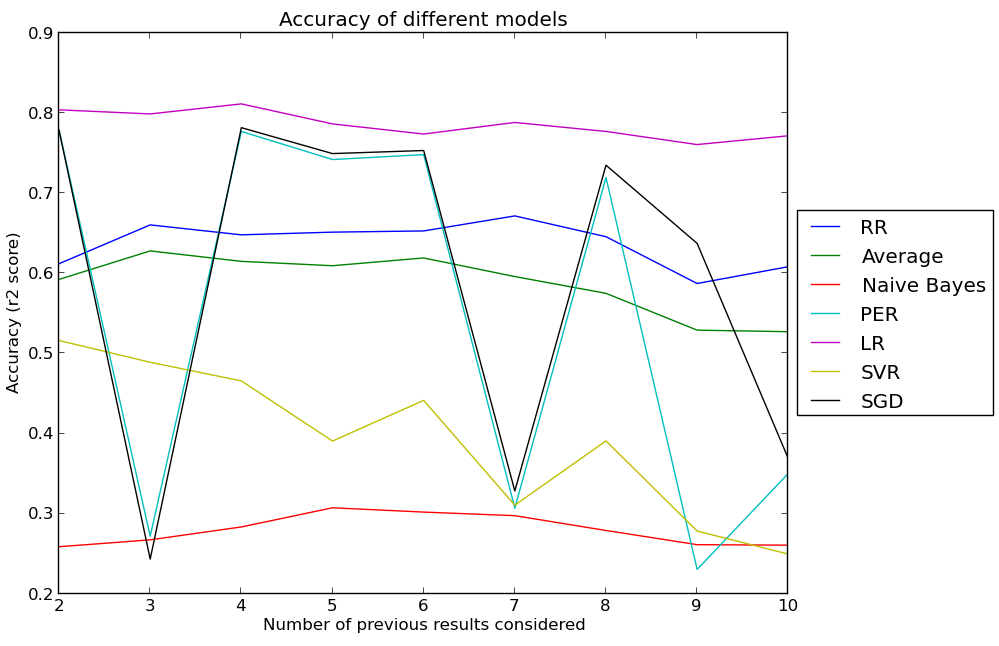
\includegraphics[width=1\textwidth]{comparison.png}
\caption{Comparison of different machine learning methods comparing their accuracy against the number of previous exercises considered}
\label{fig:comparison}
\end{figure}

%\subsubsection{Calibration}

\section{What next?}
In the next few weeks the system will be completed so that is fully functional for user testing.

\subsection{Integrating with Infandango}
To integrate with Infandango the model must be given the recent scores in order to update their predicted score and this must be used by the frontend to be displayed in some way.

\subsubsection{Database}
The functionality has already been written which queries the database for the most recent questions. It would be possible to do this without querying the database (store each new question in some temporary place) but for the limited amount of testing being performed any possible speed decrease (database queries can be slow) can be ignored. What is left is to put the code in the relevant place within the system.

\subsubsection{Frontend}
This is the area which will require the most work. The first step is to decide on the preferred design: how the predicted score will be displayed. When a number of designs have been drafted a group of students who used the system last year will be asked for which design they prefer. These designs are likely to be very visually, with little or no numbers. This is with the aim to abstract away from the marks being received and instead give the user an idea of how well they are performing: should they be working harder or are at a good stage right now?
\\
When a design is decided the placement of the widget will need to be decided. It is likely to be placed on the side bar which contains the list of weeks and questions.
